\section{Discussion} \label{Sec: Discussion}
\subsection{Total IR LF} \label{Sec: Bolometric IR LF}

\begin{figure*}
    \centering
    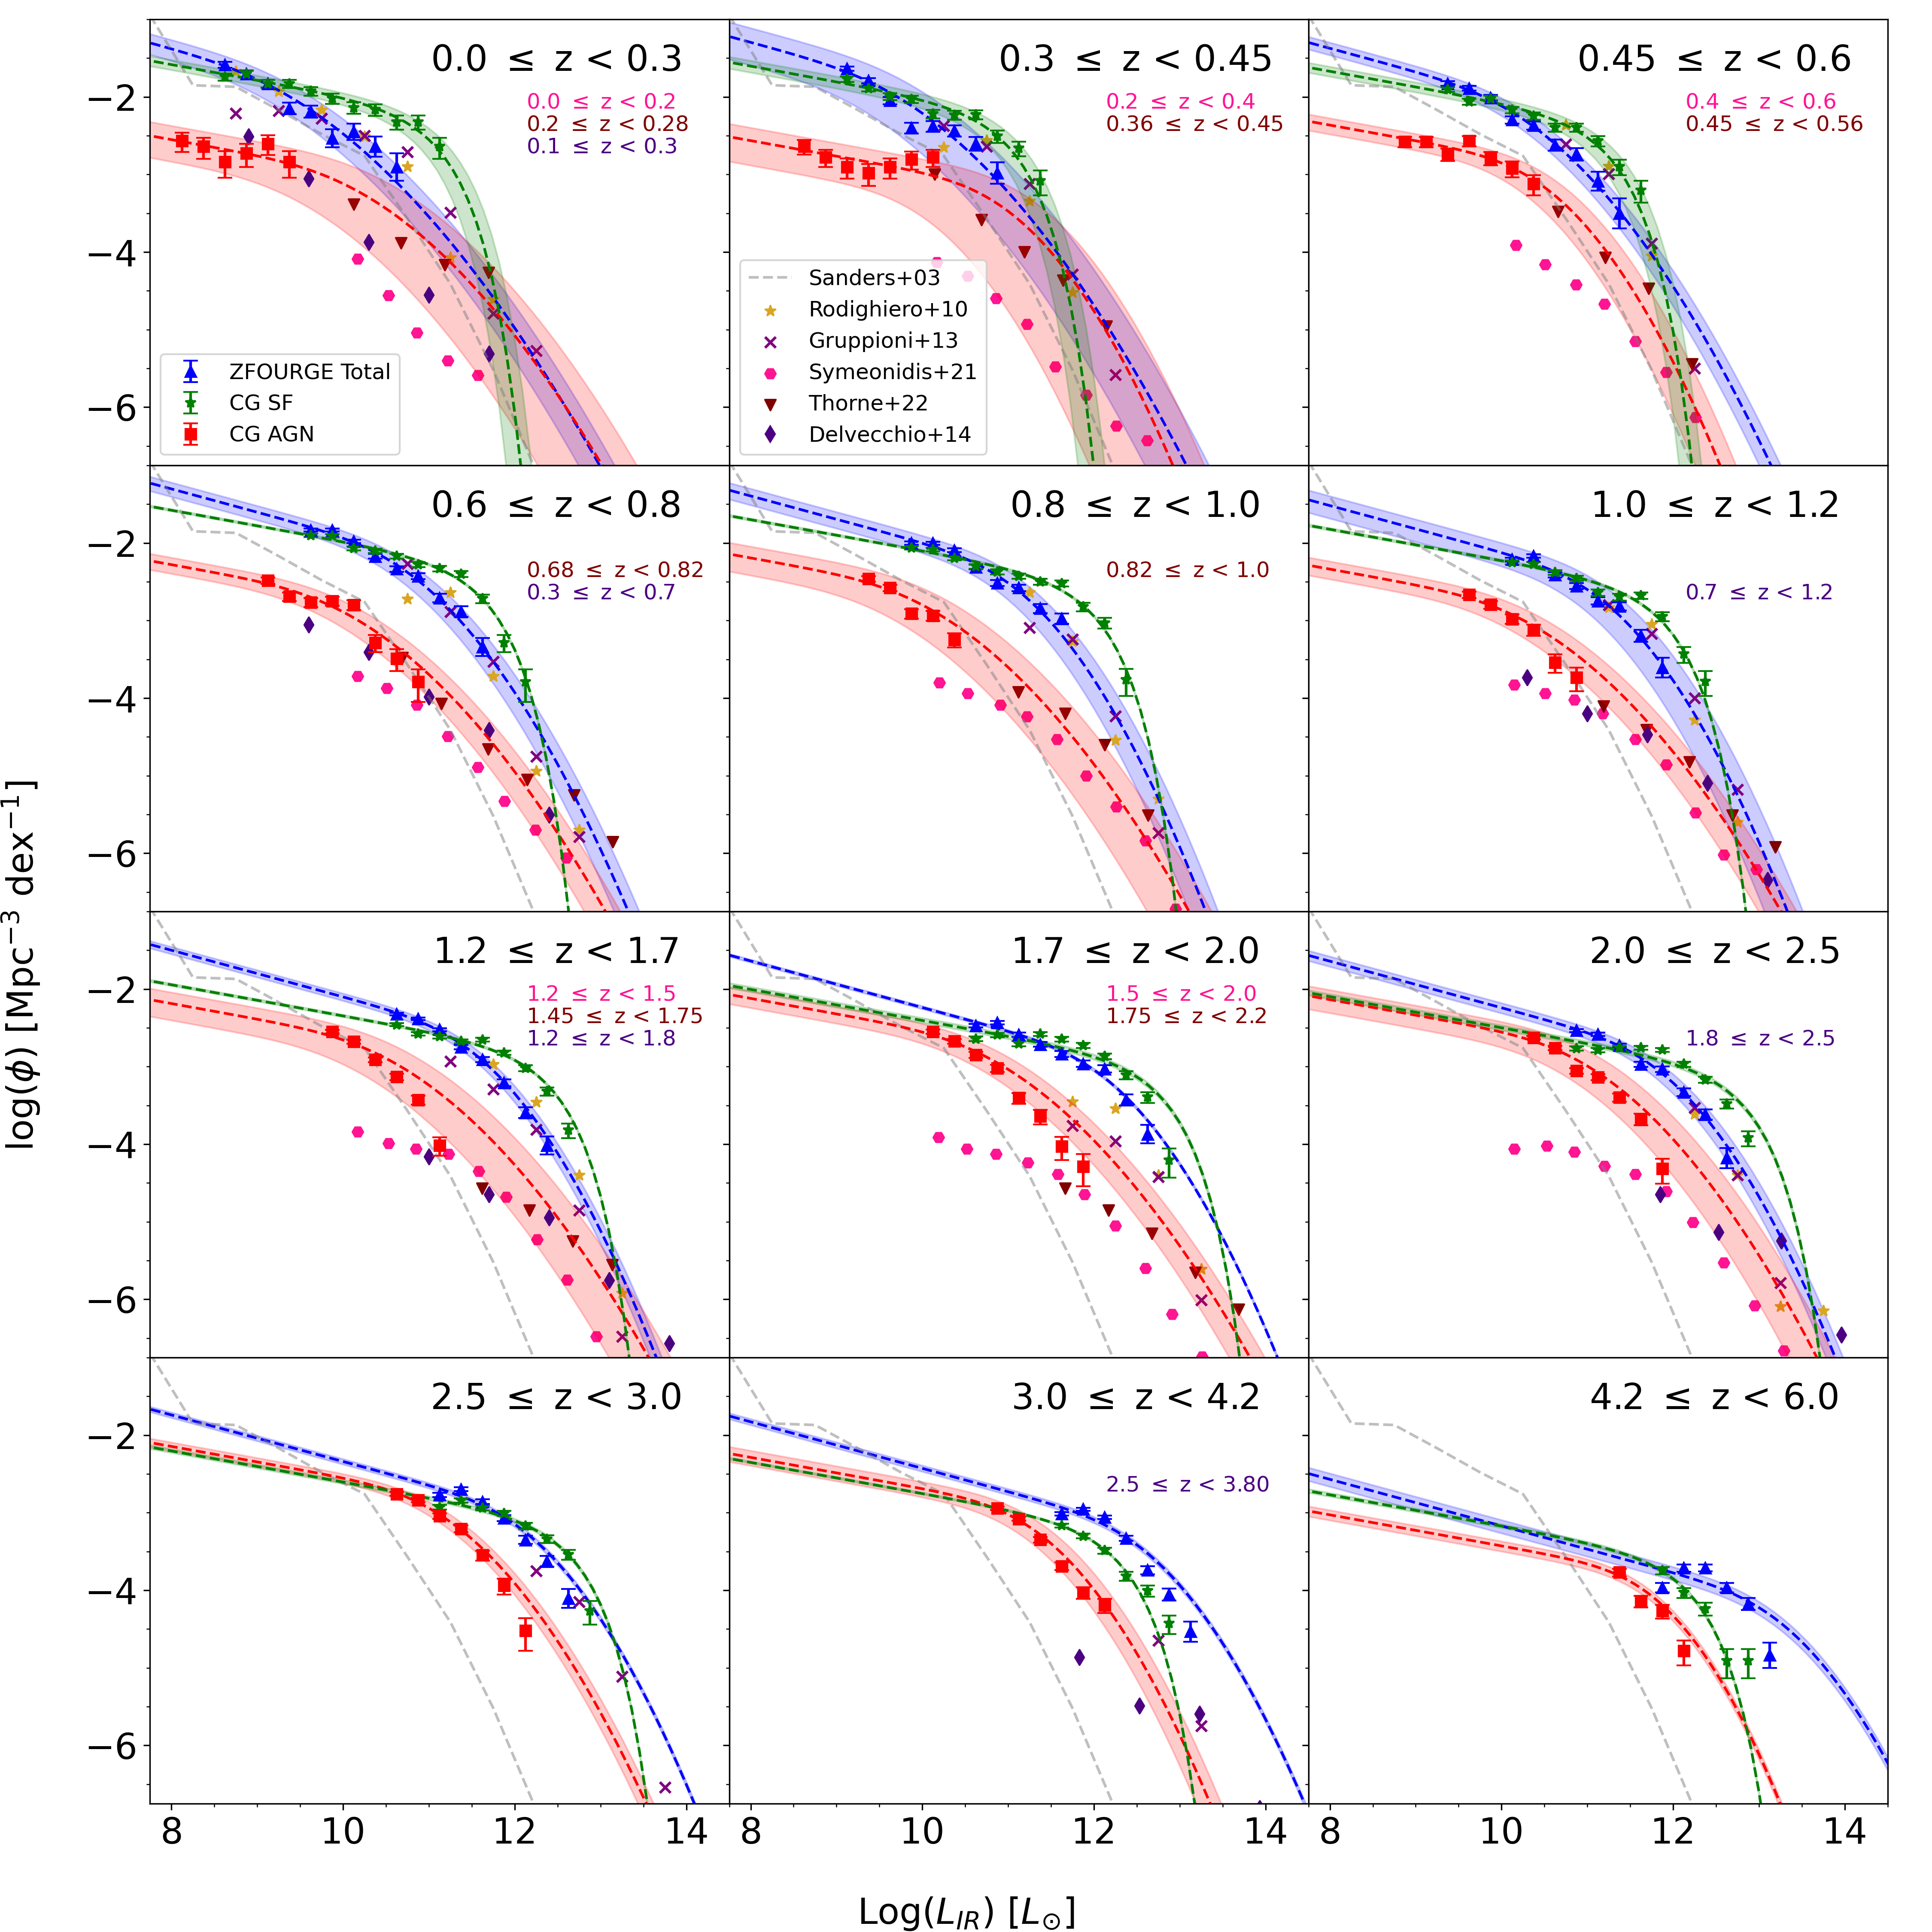
\includegraphics[width=\textwidth]{Figures/LF.png}
    \caption{The luminosity functions of major galaxy populations in ZFOURGE and CIGALE calculated using the Vmax method. The dark blue triangles present the ZFOURGE total IR (8-1000$\mu$m) LF. The CIGALE SF and AGN LFs are the green stars and red squares, respectively. The blue, red, and green dashed lines show the best fit Saunders function \citep{saunders_60-mum_1990} to the ZFOURGE, CIGALE AGN, and CIGALE SF, respectively. The shaded regions represent the functional fit errors. The luminosity completeness limit of each redshift bin is where we stop displaying fainter $\phi$ values. Where possible, comparable literature results are also shown. Cyan colours refer to literature SF/total LF and pink literature AGN. The local \cite{sanders_iras_2003} luminosity function is shown across all redshift bins as the grey dashed line. \cite{rodighiero_mid-_2010} is shown as cyan filled stars from $0 < z < 2.5$, \cite{gruppioni_herschel_2013} as cyan crosses from $0 < z < 4.2$, \cite{symeonidis_agn_2021} AGN as pink hexagons, \cite{thorne_deep_2022} AGN as pink squares, \cite{delvecchio_tracing_2014} AGN as pink diamonds. All compared literature sources use $8-1000 \mu m$ IR luminosity. Differing redshift bins are colour-labelled accordingly.}
    \label{Fig: Bolometric IR LF}
\end{figure*}

\begin{landscape}
    \begin{table*}
    \begin{center}
    \caption{ZFOURGE total IR (8-1000$\mu$m) LF $\phi$ values.}
    \label{Tab: ZF LF}
    \begin{tabular}{@{}ccccccc@{}}
        \toprule
        $\log_{10}(L_{IR}/L_{\odot})$ & 0.00 $\leq z <$ 0.30 & 0.30 $\leq z <$ 0.45 & 0.45 $\leq z <$ 0.60 & 0.60 $\leq z <$ 0.80 & 0.80 $\leq z <$ 1.00 & 1.00 $\leq z <$ 1.20 \\
        \hline
         8.50 --  8.75 & -1.58 $\pm$ 0.20 & - & - & - & - & - \\
         8.75 --  9.00 & -1.70 $\pm$ 0.26 & - & - & - & - & - \\
         9.00 --  9.25 & -1.82 $\pm$ 0.27 & -1.64 $\pm$ 0.26 & - & - & - & - \\
         9.25 --  9.50 & -2.15 $\pm$ 0.42 & -1.79 $\pm$ 0.31 & -1.82 $\pm$ 0.15 & - & - & - \\
         9.50 --  9.75 & -2.16 $\pm$ 0.26 & -2.05 $\pm$ 0.45 & -1.89 $\pm$ 0.27 & - & - & - \\
         9.75 -- 10.00 & -2.51 $\pm$ 0.42 & -2.37 $\pm$ 0.57 & -2.01 $\pm$ 0.24 & -1.83 $\pm$ 0.20 & - & - \\
        10.00 -- 10.25 & -2.43 $\pm$ 0.25 & -2.37 $\pm$ 0.25 & -2.29 $\pm$ 0.42 & -1.97 $\pm$ 0.20 & -2.00 $\pm$ 0.21 & - \\
        10.25 -- 10.50 & -2.60 $\pm$ 0.24 & -2.41 $\pm$ 0.17 & -2.34 $\pm$ 0.33 & -2.16 $\pm$ 0.32 & -2.09 $\pm$ 0.21 & -2.16 $\pm$ 0.22 \\
        10.50 -- 10.75 & -2.78 $\pm$ 0.43 & -2.58 $\pm$ 0.30 & -2.61 $\pm$ 0.31 & -2.32 $\pm$ 0.27 & -2.30 $\pm$ 0.28 & -2.41 $\pm$ 0.24 \\
        10.75 -- 11.00 & -2.90 $\pm$ 0.39 & -2.94 $\pm$ 0.67 & -2.72 $\pm$ 0.46 & -2.41 $\pm$ 0.21 & -2.50 $\pm$ 0.38 & -2.53 $\pm$ 0.31 \\
        11.00 -- 11.25 & -                & -3.28 $\pm$ 0.81 & -3.09 $\pm$ 0.50 & -2.65 $\pm$ 0.36 & -2.53 $\pm$ 0.24 & -2.71 $\pm$ 0.23 \\
        11.25 -- 11.50 & -                & -                & -3.25 $\pm$ 0.64 & -2.80 $\pm$ 0.41 & -2.79 $\pm$ 0.36 & -2.75 $\pm$ 0.24 \\
        11.50 -- 11.75 & -                & -                & -                & -3.15 $\pm$ 0.56 & -2.89 $\pm$ 0.38 & -3.10 $\pm$ 0.38 \\
        11.75 -- 12.00 & -                & -                & -                & -                & -3.76 $\pm$ 1.91 & -3.48 $\pm$ 0.97 \\
        \hline
        $\log_{10}(L_{IR}/L_{\odot})$ & 1.20 $\leq z <$ 1.70 & 1.70 $\leq z <$ 2.00 & 2.00 $\leq z <$ 2.50 & 2.50 $\leq z <$ 3.00 & 3.00 $\leq z <$ 4.20 & 4.20 $\leq z <$ 6.00  \\
        \hline
        10.50 -- 10.75 & -2.32 $\pm$ 0.13 & - & - & - & - & - \\
        10.75 -- 11.00 & -2.37 $\pm$ 0.21 & -2.43 $\pm$ 0.19 & -2.53 $\pm$ 0.14 & - & - & - \\
        11.00 -- 11.25 & -2.51 $\pm$ 0.24 & -2.59 $\pm$ 0.20 & -2.58 $\pm$ 0.22 & - & - & - \\
        11.25 -- 11.50 & -2.72 $\pm$ 0.34 & -2.70 $\pm$ 0.21 & -2.72 $\pm$ 0.23 & -2.69 $\pm$ 0.21 & - & - \\
        11.50 -- 11.75 & -2.87 $\pm$ 0.38 & -2.83 $\pm$ 0.16 & -2.95 $\pm$ 0.29 & -2.85 $\pm$ 0.21 & - & - \\
        11.75 -- 12.00 & -3.14 $\pm$ 0.44 & -2.94 $\pm$ 0.18 & -3.02 $\pm$ 0.25 & -3.04 $\pm$ 0.35 & -2.96 $\pm$ 0.17 & - \\
        12.00 -- 12.25 & -3.49 $\pm$ 0.71 & -2.99 $\pm$ 0.26 & -3.27 $\pm$ 0.40 & -3.29 $\pm$ 0.45 & -3.05 $\pm$ 0.21 & - \\
        12.25 -- 12.50 & -3.82 $\pm$ 0.72 & -3.31 $\pm$ 0.51 & -3.52 $\pm$ 0.51 & -3.58 $\pm$ 0.66 & -3.32 $\pm$ 0.41 & -3.71 $\pm$ 0.24 \\
        12.50 -- 12.75 & -                & -3.81 $\pm$ 1.02 & -3.97 $\pm$ 0.91 & -3.84 $\pm$ 0.57 & -3.72 $\pm$ 0.73 & -3.97 $\pm$ 0.35 \\
        12.75 -- 13.00 & -                & -                & -                & -                & -3.98 $\pm$ 0.52 & -4.14 $\pm$ 0.39 \\
        13.00 -- 13.25 & -                & -                & -                & -                & -4.32 $\pm$ 0.54 & -4.84 $\pm$ 1.35 \\
        13.25 -- 13.50 & -                & -                & -                & -                & -4.80 $\pm$ 0.87 & - \\
        \bottomrule
    \end{tabular}
    \end{center}
    \textbf{Note}: Luminosity bin $\phi$ values are centred.
    \end{table*}
\end{landscape}

\begin{landscape}
    \begin{table*}
    \begin{center}
    \caption{CIGALE AGN LF $\phi$ values.}
    \label{Tab: CG AGN LF}
    \begin{tabular}{@{}ccccccc@{}}
        \toprule
        $\log_{10}(L_{IR}/L_{\odot})$ & 0.00 $\leq z <$ 0.30 & 0.30 $\leq z <$ 0.45 & 0.45 $\leq z <$ 0.60 & 0.60 $\leq z <$ 0.80 & 0.80 $\leq z <$ 1.00 & 1.00 $\leq z <$ 1.20 \\
        \hline
         8.00 --  8.25 & -2.32 $\pm$ 0.28 & -                & -                & -                & -                & - \\
         8.25 --  8.50 & -2.54 $\pm$ 0.17 & -2.30 $\pm$ 0.24 & -                & -                & -                & - \\
         8.50 --  8.75 & -2.64 $\pm$ 0.32 & -2.48 $\pm$ 0.18 & -                & -                & -                & - \\
         8.75 --  9.00 & -3.08 $\pm$ 0.56 & -2.57 $\pm$ 0.23 & -2.36 $\pm$ 0.18 & -                & -                & - \\
         9.00 --  9.25 & -2.68 $\pm$ 0.19 & -2.90 $\pm$ 0.43 & -2.50 $\pm$ 0.19 & -2.31 $\pm$ 0.22 & -                & - \\
         9.25 --  9.50 & -2.84 $\pm$ 0.23 & -2.94 $\pm$ 0.22 & -2.70 $\pm$ 0.35 & -2.47 $\pm$ 0.23 & -2.28 $\pm$ 0.26 & - \\
         9.50 --  9.75 & -2.98 $\pm$ 0.26 & -2.94 $\pm$ 0.14 & -2.60 $\pm$ 0.15 & -2.71 $\pm$ 0.56 & -2.40 $\pm$ 0.28 & -2.42 $\pm$ 0.25 \\
         9.75 -- 10.00 & -2.98 $\pm$ 0.35 & -2.98 $\pm$ 0.14 & -2.72 $\pm$ 0.18 & -2.67 $\pm$ 0.20 & -2.67 $\pm$ 0.63 & -2.58 $\pm$ 0.24 \\
        10.00 -- 10.25 & -                & -2.87 $\pm$ 0.31 & -2.88 $\pm$ 0.20 & -2.76 $\pm$ 0.22 & -2.76 $\pm$ 0.53 & -2.78 $\pm$ 0.59 \\
        10.25 -- 10.50 & -                & -                & -3.09 $\pm$ 0.37 & -3.09 $\pm$ 0.43 & -3.08 $\pm$ 0.66 & -2.91 $\pm$ 0.65 \\
        10.50 -- 10.75 & -                & -                & -3.50 $\pm$ 0.53 & -3.31 $\pm$ 0.30 & -3.76 $\pm$ 1.49 & -3.20 $\pm$ 0.50 \\
        10.75 -- 11.00 & -                & -                & -                & -3.45 $\pm$ 0.27 & -4.01 $\pm$ 0.58 & -3.46 $\pm$ 0.56 \\
        11.00 -- 11.25 & -                & -                & -                & -3.79 $\pm$ 0.50 & -                & -3.69 $\pm$ 0.46 \\
        \hline
        $\log_{10}(L_{IR}/L_{\odot})$ & 1.20 $\leq z <$ 1.70 & 1.70 $\leq z <$ 2.00 & 2.00 $\leq z <$ 2.50 & 2.50 $\leq z <$ 3.00 & 3.00 $\leq z <$ 4.20 & 4.20 $\leq z <$ 6.00  \\
        \hline
         9.75 -- 10.00 & -2.23 $\pm$ 0.32 & -                & -                & -                & -                & - \\
        10.00 -- 10.25 & -2.41 $\pm$ 0.30 & -2.18 $\pm$ 0.31 & -                & -                & -                & - \\
        10.25 -- 10.50 & -2.69 $\pm$ 0.45 & -2.35 $\pm$ 0.29 & -2.26 $\pm$ 0.31 & -2.48 $\pm$ 0.13 & -                & - \\
        10.50 -- 10.75 & -2.87 $\pm$ 0.97 & -2.62 $\pm$ 0.23 & -2.54 $\pm$ 0.28 & -2.38 $\pm$ 0.25 & -                & - \\
        10.75 -- 11.00 & -3.18 $\pm$ 1.27 & -2.85 $\pm$ 1.34 & -2.79 $\pm$ 0.64 & -2.60 $\pm$ 0.24 & -2.61 $\pm$ 0.27 & - \\
        11.00 -- 11.25 & -3.67 $\pm$ 1.56 & -3.15 $\pm$ 1.09 & -2.96 $\pm$ 1.07 & -3.83 $\pm$ 0.54 & -2.84 $\pm$ 0.29 & - \\
        11.25 -- 11.50 & -3.93 $\pm$ 0.86 & -3.47 $\pm$ 0.83 & -3.18 $\pm$ 0.67 & -3.04 $\pm$ 0.73 & -3.19 $\pm$ 0.87 & -3.29 $\pm$ 0.33 \\
        11.50 -- 11.75 & -4.12 $\pm$ 0.36 & -3.81 $\pm$ 0.75 & -3.56 $\pm$ 0.74 & -3.39 $\pm$ 0.70 & -3.57 $\pm$ 1.34 & -3.47 $\pm$ 0.34 \\
        11.75 -- 12.00 & -                & -4.14 $\pm$ 0.61 & -3.90 $\pm$ 0.73 & -3.79 $\pm$ 0.86 & -3.98 $\pm$ 1.13 & -3.94 $\pm$ 0.29 \\
        12.00 -- 12.25 & -                & -                & -4.44 $\pm$ 0.90 & -4.22 $\pm$ 0.86 & -4.06 $\pm$ 0.42 & -4.22 $\pm$ 1.54 \\
        12.25 -- 12.50 & -                & -                & -                & -                & -4.57 $\pm$ 0.85 & -4.64 $\pm$ 1.74 \\
        \bottomrule
    \end{tabular}
    \end{center}
    \textbf{Note}: Luminosity bin $\phi$ values are centred.
    \end{table*}
\end{landscape}

\begin{landscape}
    \begin{table*}
    \begin{center}
    \caption{CIGALE SF LF $\phi$ values.}
    \label{Tab: CG SF LF}
    \begin{tabular}{@{}ccccccc@{}}
        \toprule
        $\log_{10}(L_{IR}/L_{\odot})$ & 0.00 $\leq z <$ 0.30 & 0.30 $\leq z <$ 0.45 & 0.45 $\leq z <$ 0.60 & 0.60 $\leq z <$ 0.80 & 0.80 $\leq z <$ 1.00 & 1.00 $\leq z <$ 1.20 \\
        \hline
         8.50 --  8.75 & -1.41 $\pm$ 0.05 & - & - & - & - & - \\
         8.75 --  9.00 & -1.44 $\pm$ 0.10 & - & - & - & - & - \\
         9.00 --  9.25 & -1.59 $\pm$ 0.15 & -1.50 $\pm$ 0.16 & - & - & - & - \\
         9.25 --  9.50 & -1.65 $\pm$ 0.12 & -1.65 $\pm$ 0.16 & -1.60 $\pm$ 0.15 & - & - & - \\
         9.50 --  9.75 & -1.84 $\pm$ 0.20 & -1.80 $\pm$ 0.18 & -1.79 $\pm$ 0.17 & -1.61 $\pm$ 0.10 & - & - \\
         9.75 -- 10.00 & -1.97 $\pm$ 0.15 & -1.91 $\pm$ 0.17 & -1.83 $\pm$ 0.14 & -1.68 $\pm$ 0.14 & -1.74 $\pm$ 0.15 & - \\
        10.00 -- 10.25 & -2.09 $\pm$ 0.12 & -2.12 $\pm$ 0.20 & -2.06 $\pm$ 0.24 & -1.87 $\pm$ 0.18 & -1.86 $\pm$ 0.16 & -1.95 $\pm$ 0.16 \\
        10.25 -- 10.50 & -2.13 $\pm$ 0.10 & -2.20 $\pm$ 0.08 & -2.20 $\pm$ 0.18 & -1.98 $\pm$ 0.15 & -2.05 $\pm$ 0.24 & -2.09 $\pm$ 0.17 \\
        10.50 -- 10.75 & -2.23 $\pm$ 0.12 & -2.19 $\pm$ 0.11 & -2.36 $\pm$ 0.14 & -2.09 $\pm$ 0.14 & -2.21 $\pm$ 0.17 & -2.25 $\pm$ 0.19 \\
        10.75 -- 11.00 & -2.30 $\pm$ 0.17 & -2.48 $\pm$ 0.26 & -2.36 $\pm$ 0.10 & -2.22 $\pm$ 0.12 & -2.30 $\pm$ 0.11 & -2.38 $\pm$ 0.16 \\
        11.00 -- 11.25 & -2.60 $\pm$ 0.41 & -2.57 $\pm$ 0.27 & -2.53 $\pm$ 0.22 & -2.27 $\pm$ 0.08 & -2.40 $\pm$ 0.08 & -2.58 $\pm$ 0.22 \\
        11.25 -- 11.50 & -                & -3.08 $\pm$ 0.61 & -2.86 $\pm$ 0.45 & -2.36 $\pm$ 0.16 & -2.43 $\pm$ 0.07 & -2.65 $\pm$ 0.18 \\
        11.50 -- 11.75 & -                & -                & -3.20 $\pm$ 0.44 & -2.62 $\pm$ 0.38 & -2.44 $\pm$ 0.13 & -2.60 $\pm$ 0.22 \\
        11.75 -- 12.00 & -                & -                & -                & -3.19 $\pm$ 0.80 & -2.75 $\pm$ 0.32 & -2.87 $\pm$ 0.38 \\
        12.00 -- 12.25 & -                & -                & -                & -3.71 $\pm$ 0.68 & -2.98 $\pm$ 0.38 & -3.36 $\pm$ 0.59 \\
        12.25 -- 12.50 & -                & -                & -                & -                & -3.71 $\pm$ 1.21 & -3.57 $\pm$ 0.36 \\
        \hline
        $\log_{10}(L_{IR}/L_{\odot})$ & 1.20 $\leq z <$ 1.70 & 1.70 $\leq z <$ 2.00 & 2.00 $\leq z <$ 2.50 & 2.50 $\leq z <$ 3.00 & 3.00 $\leq z <$ 4.20 & 4.20 $\leq z <$ 6.00  \\
        \hline
        10.25 -- 10.50 & -2.15 $\pm$ 0.11 & - & - & - & - & - \\
        10.50 -- 10.75 & -2.23 $\pm$ 0.16 & -2.35 $\pm$ 0.05 & - & - & - & - \\
        10.75 -- 11.00 & -2.41 $\pm$ 0.18 & -2.38 $\pm$ 0.09 & -2.47 $\pm$ 0.07 & - & - & - \\
        11.00 -- 11.25 & -2.51 $\pm$ 0.11 & -2.53 $\pm$ 0.24 & -2.54 $\pm$ 0.08 & - & - & - \\
        11.25 -- 11.50 & -2.56 $\pm$ 0.05 & -2.47 $\pm$ 0.10 & -2.57 $\pm$ 0.06 & -2.62 $\pm$ 0.13 & -2.93 $\pm$ 0.07 & - \\
        11.50 -- 11.75 & -2.57 $\pm$ 0.09 & -2.57 $\pm$ 0.12 & -2.61 $\pm$ 0.08 & -2.77 $\pm$ 0.15 & -2.95 $\pm$ 0.10 & - \\
        11.75 -- 12.00 & -2.73 $\pm$ 0.19 & -2.68 $\pm$ 0.15 & -2.69 $\pm$ 0.15 & -2.87 $\pm$ 0.18 & -3.09 $\pm$ 0.22 & -3.52 $\pm$ 0.25 \\
        12.00 -- 12.25 & -2.92 $\pm$ 0.25 & -2.81 $\pm$ 0.19 & -2.90 $\pm$ 0.22 & -3.05 $\pm$ 0.22 & -3.31 $\pm$ 0.32 & -3.80 $\pm$ 0.35 \\
        12.25 -- 12.50 & -3.23 $\pm$ 0.41 & -3.06 $\pm$ 0.29 & -3.10 $\pm$ 0.28 & -3.23 $\pm$ 0.23 & -3.64 $\pm$ 0.38 & -4.07 $\pm$ 0.40 \\
        12.50 -- 12.75 & -3.68 $\pm$ 0.62 & -3.33 $\pm$ 0.45 & -3.38 $\pm$ 0.36 & -3.46 $\pm$ 0.38 & -3.88 $\pm$ 0.34 & -4.57 $\pm$ 0.72 \\
        12.75 -- 13.00 & -                & -4.14 $\pm$ 1.34 & -3.82 $\pm$ 0.55 & -4.18 $\pm$ 1.19 & -4.25 $\pm$ 0.52 & -4.91 $\pm$ 0.80 \\
        13.00 -- 13.25 & -                & -                & -4.44 $\pm$ 1.04 & -                & -4.67 $\pm$ 0.59 & -4.98 $\pm$ 0.32 \\
        \bottomrule
    \end{tabular}
    \end{center}
    % \textbf{Note}: Luminosity bin $\phi$ values are centred.
    \end{table*}
\end{landscape}

Figure \ref{Fig: Bolometric IR LF} presents the total IR LFs derived from the ZFOURGE and CIGALE samples. Different luminosity bins are used when compared to \cref{Sec: Luminosity Functions Chapter}. Specifically, the relative size of each luminosity bin has been cut in half. This has the effect of introducing more bins into our analysis so the applied fitting routine can constrain a more accurate fit. This comparison allows us to explore the evolution of total IR emission and the individual contributions from SF and AGN across twelve redshift bins from $0 \leq z < 6$. By comparing the LF from ZFOURGE with the decomposed SF and AGN LFs from CIGALE, we aim to better understand the distinct roles of SF and AGN activity in galaxy evolution over cosmic time. To model these LFs, we employ \texttt{scipy.optimize.curve\_fit} \citep{virtanen_scipy_2020} which performs non-linear least squares fitting, optimising model parameters by minimising the difference between the model and observed data. 

Relative 1$\sigma$ parameter dispersion errors were calculated using \texttt{np.sqrt(np.diag(pcov))} from \texttt{NumPy} \citep{harris_array_2020}, which relates the covariance of the best-fit parameters. Additionally, the fitting routine is applied to a ``worst-case" upper and lower luminosity based on the accrued errors of redshift, $L_{IR}$, and FIR availability. The errors from these ``worst cases" are then added in quadrature to the uncertainty of the parameters. The shaded regions shown in Figure \ref{Fig: Bolometric IR LF} represent the combined uncertainties, including observational errors (photometric redshifts, LIR, and FIR limitations) and fitting uncertainties (including covariance between fitted LF parameters). These regions thus reflect the plausible range in the LF shape given the data.

It is important to note that the LFs derived in this work apply to the population of galaxies detectable within a near-infrared selection framework, as discussed in Section \ref{Sec: Galaxy LF Selection}. As such, they may underrepresent the most heavily obscured galaxies and AGN, and likely constitute a lower limit on the true space density of dust-obscured systems. This limitation is expected to primarily affect the faint end of the luminosity function, where obscured but intrinsically faint galaxies are most likely to be missed. However, the bright end, which is dominated by luminous systems, is less sensitive to this bias and should remain largely representative. As such, our luminosity functions should be regarded as conservative lower limits, particularly at lower luminosities. Again, as mentioned in Sections \ref{Sec: IR_Luminosity} and \ref{Sec: FIR Constraints}, we include and account for FIR errors to capture the true shape of each LF inside our uncertainty.

\subsubsection{ZFOURGE} \label{Sec: ZF Total Discussion}
Focusing first on the ZFOURGE data, we compare our results with \cite{rodighiero_mid-_2010} and \cite{gruppioni_herschel_2013}. We also compare our results with \cite{huang_local_2007, caputi_infrared_2007, fu_decomposing_2010} but avoid cluttering figure \ref{Fig: Bolometric IR LF} with these disjointed redshift bins from the literature. Across all redshift bins (except the most local), we consistently see that the ZFOURGE number density ($\phi$) values in blue extend much fainter than the rest of the literature, showcasing ZFOURGE's ability to probe to fainter luminosities. However, there remains room to improve the constraints at the faint end of the ZFOURGE LF. Extending the analysis by an additional order of magnitude fainter in each redshift bin would significantly enhance our ability to constrain the faint-end slope.

We do not compare the CIGALE Total LF to the ZFOURGE LF. This is because the CIGALE Total LF is practically identical to the CIGALE SF LF and would clutter Figure \ref{Fig: Bolometric IR LF}. Instead, we present the LFs of ZFOURGE, CIGALE Total, and CIGALE components in Appendix A at the end of this article.

\begin{figure}
    \centering
    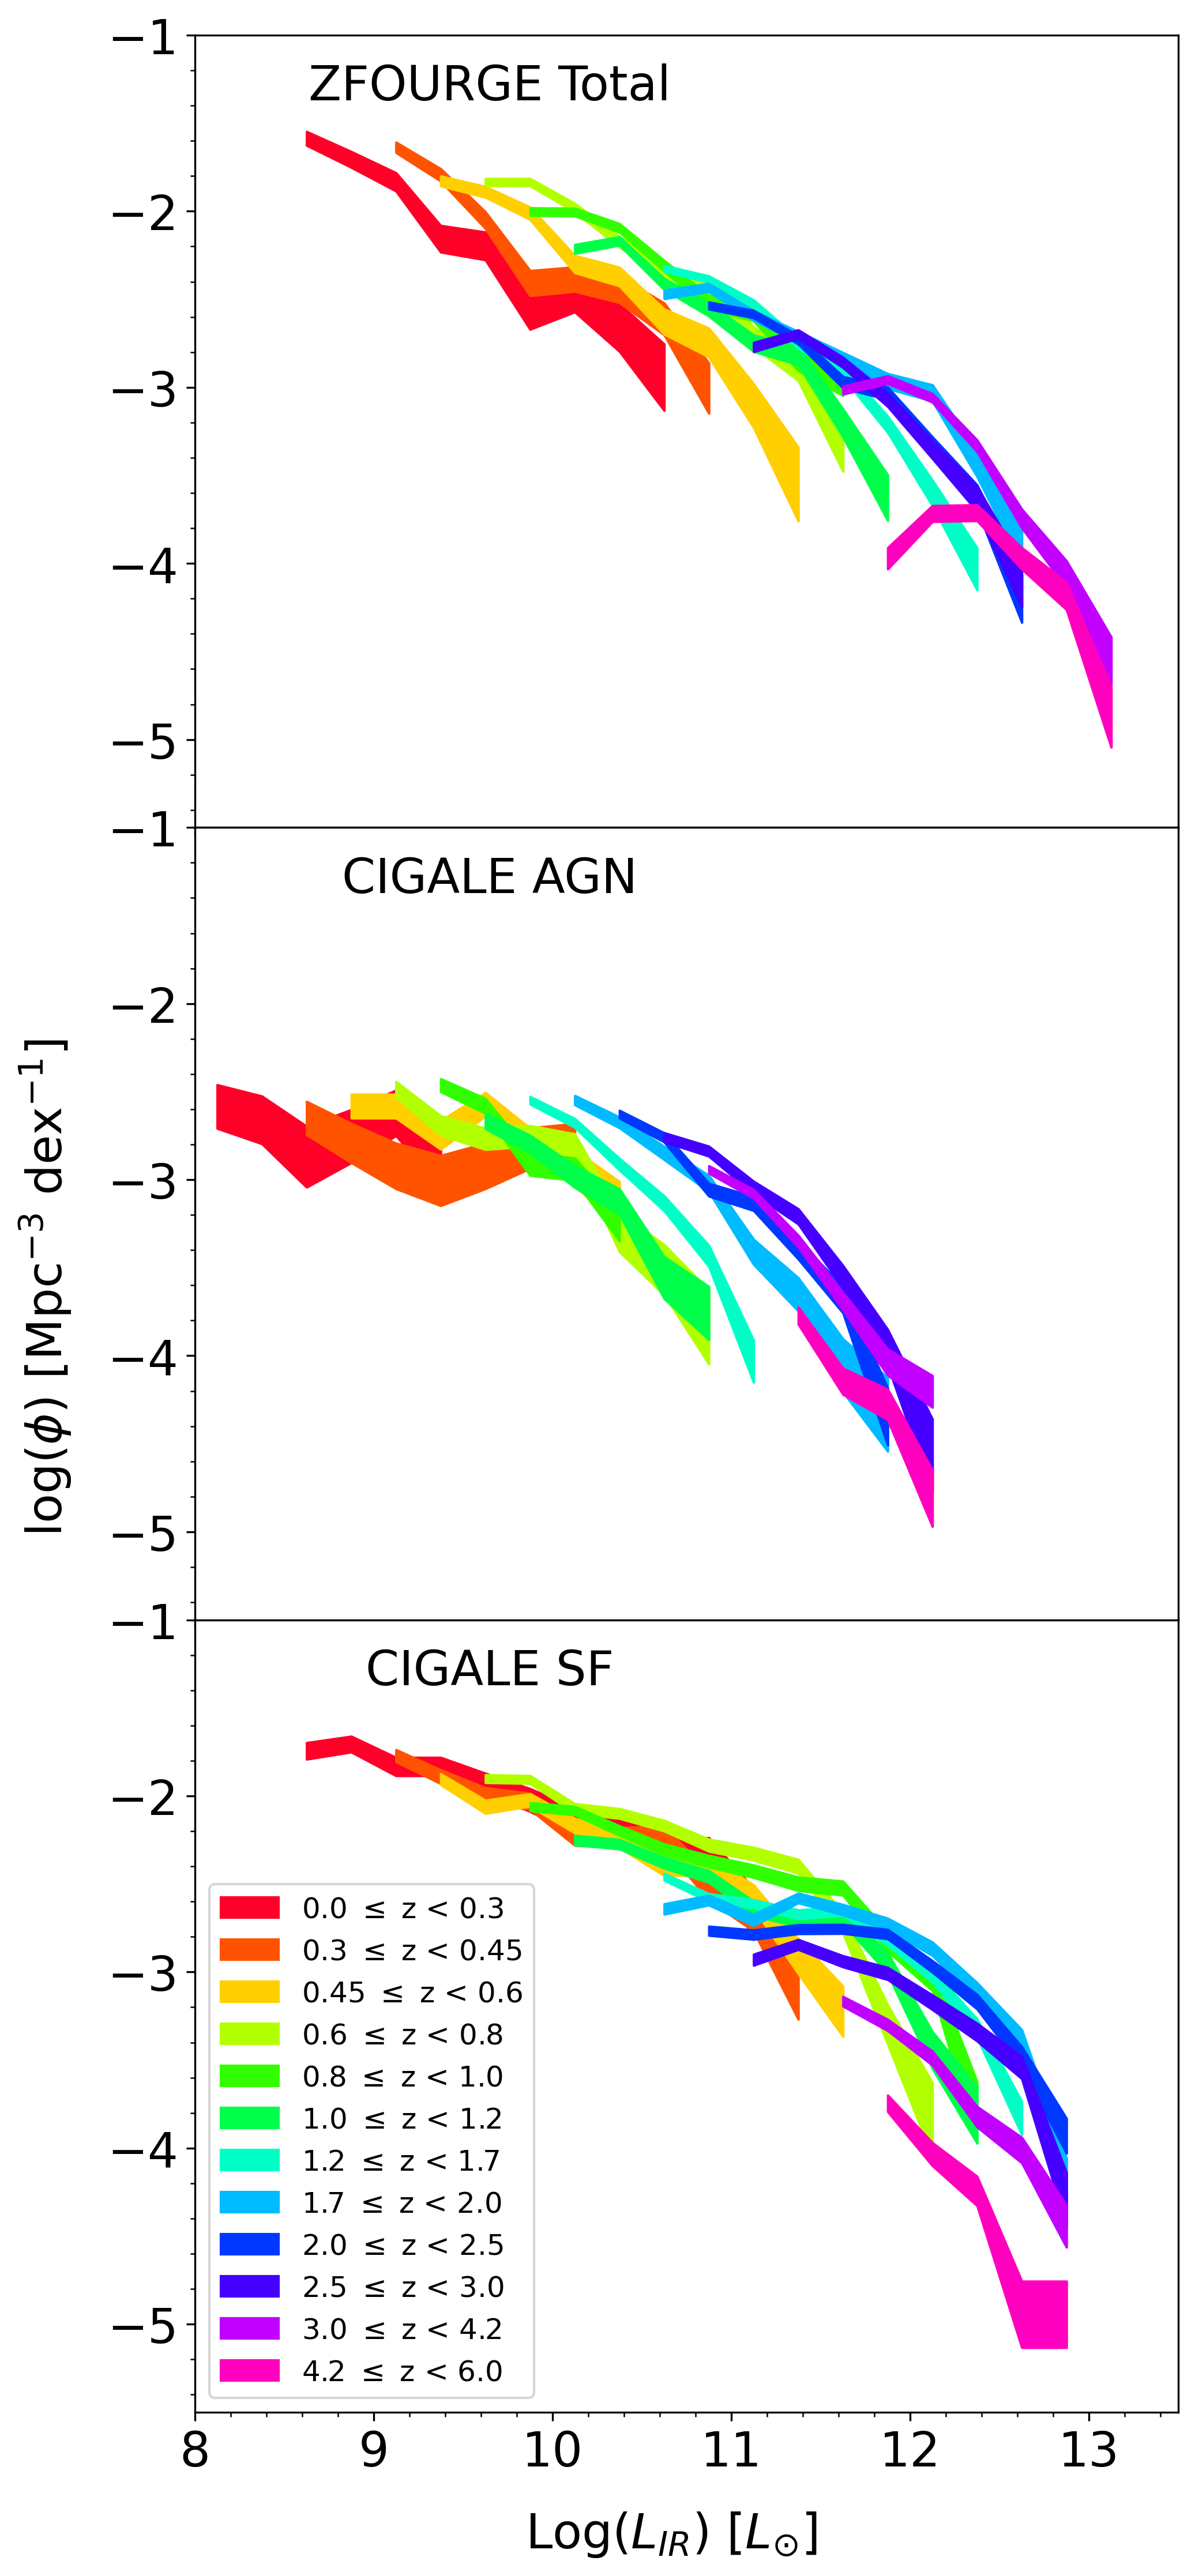
\includegraphics[width=0.7\textwidth]{Figures/LF_Filled.png}
    \caption{Combined evolution of the ZFOURGE total (top), CIGALE AGN (middle), and CIGALE SF (bottom) luminosity functions shown in figure \ref{Fig: Bolometric IR LF}. The redshift evolution of each binned LF is easier to visualise. Data points are shaded between the uncertainties and coloured by redshift bin.}
    \label{Fig: LF Filled}
\end{figure}

Our ZFOURGE results agree very well with the literature in all bins except $1.7 \leq z < 2$ and $3.0 \leq z < 4.2$. In these redshift bins, ZFOURGE results show $\phi$ values $\approx$ 0.2 --- 0.5 dex higher across all luminosity bins when compared to \cite{rodighiero_mid-_2010} and \cite{gruppioni_herschel_2013}. We posit that ZFOURGE is detecting fainter sources in these redshift bins than previously observed. From $1.7 \leq z < 2$, both \cite{rodighiero_mid-_2010} and \cite{gruppioni_herschel_2013} show a drop in their faintest luminosity bins. The fact that both \cite{gruppioni_herschel_2013} and \cite{rodighiero_mid-_2010} see a drop from $1.7 \leq z < 2$ is intriguing. This issue does not appear in neighbouring redshift bins or other redshift bins. \cite{rodighiero_mid-_2010} utilises multiwavelength Spitzer observations, whereas \cite{gruppioni_herschel_2013} uses Herschel/PACS data to estimate the total IR LF. Given that this exists across multiple surveys and instruments, it remains to be seen why a drop in the $1.7 \leq z < 2$ redshift bin exists. Our ZFOURGE results, on the other hand, do not show this drop. Luminosity bins in our final redshift bin $4.2 \leq z < 6.0$ (figure \ref{Fig: Bolometric IR LF}) show a drop along the faint end slop of our LF. Therefore, our final redshift bin $4.2 \leq z < 6.0$ is likely incomplete and should be taken as a lower limit.

\subsubsection{CIGALE AGN}
For the CIGALE AGN, we compare our results with \cite{delvecchio_tracing_2014, symeonidis_agn_2021} and \cite{thorne_deep_2022}. \cite{symeonidis_agn_2021} derives their IR AGN $\phi$ values from the hard X-ray LFs by \cite{aird_evolution_2015}. \cite{thorne_deep_2022}, who performs similar work to this analysis, uses the SED fitting code \texttt{ProSpect} \citep{leja_deriving_2017, robotham_prospect_2020} to decompose the total IR LF and recover the pure AGN component to the LF. We fit the Saunders function in red and uncertainties to our CIGALE decomposed AGN LF. We include \cite{thorne_deep_2022} AGN in our fitting process as we do not have comparatively bright AGN to constrain the bright end of the LF. 

In the first few redshift bins from $0 \leq z < 0.8$, our CIGALE AGN LF and the Saunders function fits are generally consistent with the results in the literature. However, the literature LFs tend to flatten considerably at higher redshifts and fainter luminosities. In contrast, our CIGALE AGN LFs do not flatten and instead continue to rise, suggesting that CIGALE SED decomposition is effective in isolating and recovering the AGN contribution to luminosities as faint as $10^8$ $L_{\odot}$. Furthermore, we probe fainter than \cite{thorne_deep_2022} whose faintest luminosity bins are never less than $10^{10}$ $L_{\odot}$ (when accounting for their completeness limits). Although our CIGALE AGN LF lacks $\phi$ values at the bright end, necessitating the use of \cite{thorne_deep_2022} $\phi$ values to constrain our Saunders function fits, CIGALE's ability to extend the LF to such faint luminosities provides crucial insights into the AGN population at higher redshifts. 

The ZFOURGE LF, especially at the bright end, is elevated above the CIGALE AGN LF across all redshift bins. This may result from AGN contributions that are not captured in the decomposed AGN LF due to limitations in FIR coverage and SED constraints at high luminosities. Additionally, we have shown the \cite{wuyts_fireworks_2008} method (in Section \ref{Sec: IR Density}) likely overestimates the IR luminosity at $z>3$. This is visually represented by Figure \ref{Fig: LIR vs LIR} (bottom). Furthermore, there are many fewer and fainter CIGALE AGN sources to work with at this redshift range. This reduction reflects not only the intrinsic scarcity of luminous AGN at high redshift, but also the stricter quality criteria applied during CIGALE SED fitting. As a result, the CIGALE AGN LF at the bright end may underrepresent some systems that are included in the ZFOURGE total LF, further contributing to the observed discrepancy.

Because the IR AGN identified by \cite{symeonidis_agn_2021} are derived from the hard X-ray LF presented by \cite{aird_evolution_2015}, the observed flattening at fainter luminosities is almost certainly due to X-ray emission not identifying the obscured faint AGN population. It is unclear how many IR AGN are missed by X-ray selection effects, however faint AGN are more likely to be missed \citep{frias_castillo_at_2024}. In contrast, SED fitting, as applied in our study, allows us to recover these faint AGN, providing a more complete picture of the AGN population \citep{gruppioni_modelling_2011, brown_infrared_2019, thorne_deep_2022}. Although not shown in Figure \ref{Fig: Bolometric IR LF}, the combined type-1 and type-2 AGN from \cite{symeonidis_agn_2021} show elevated number densities, particularly in the $1.2 \leq z < 2.5$ range, and align well with our CIGALE AGN results. This strong agreement underscores the robustness of our approach in isolating obscured faint AGN, especially at higher redshifts.

As the CIGALE AGN LF evolves with redshift, the faint end approaches the number density values of the CIGALE SF LF (discussed in the following subsection) at $0 \leq z < 2.5$ and nearly surpasses them at $z > 2.5$. This trend aligns with the well-known peak of the cosmic SF of galaxies above $z=2$ \citep{madau_cosmic_2014}. Conversely, the AGN fraction increases with redshift and $L_{IR}$ as noted by \cite{symeonidis_agn_2021, thorne_deep_2022} and references therein. Although our results do not yet show AGN number densities overtaking those of SF galaxies, future studies probing higher redshifts will likely reveal this transition, reflecting the dominance of AGN activity in the extremely early universe.

\subsubsection{CIGALE SF}
As seen in Figure \ref{Fig: Bolometric IR LF}, the CIGALE SF LF is elevated above the ZFOURGE and comparable literature LFs at fainter luminosities. We see a tight relationship between CIGALE SF and ZFOURGE LFs, with CIGALE SF slightly elevated above ZFOURGE in all but the highest redshift bins where AGN activity increases. Several factors could contribute to this result. Work by \cite{wu_mid-infrared_2011} has shown that the UV and optical wavelengths follow a Schechter function closely. In contrast, the IR wavelengths have a shallower exponential, which is inconsistent with a Schechter function \citep{symeonidis_what_2019}. Although our results in Figure \ref{Fig: Bolometric IR LF} show fewer luminosity bins at the bright end, we argue that CIGALE accurately isolates the SF fraction and AGN contribution to galaxy emission. 

As expected, the bright-end slope of a Schechter function is too steep to accurately describe the ZFOURGE LF \citep{wu_mid-infrared_2011}, in agreement with the literature \citep{rodighiero_mid-_2010, gruppioni_herschel_2013, symeonidis_what_2019}. Even after removing AGN-identified galaxies (552, \citealp{cowley_zfourge_2016}) and rerunning the analysis, the ZFOURGE LFs do not show an improved Schechter function fit as predicted by \cite{fu_decomposing_2010, wu_mid-infrared_2011}. The most likely reason is that \cite{cowley_zfourge_2016} only identifies the most AGN-dominated sources, leaving fainter-luminosity AGN undetected. AGN activity and SFR are tightly coupled (\citealp{alexander_what_2012} and references within), with both AGN activity and SF likely happening at the same time or offset from each other \citep{cowley_decoupled_2018}. At higher redshifts ($z > 2$), it becomes increasingly essential to disentangle AGN and SF components of galaxy emission to model galaxy evolution accurately.

\subsubsection{Combined Evolution}
In Figure \ref{Fig: LF Filled}, we show the combined evolution of the IR (8-1000$\mu$m) LFs introduced in Figure \ref{Fig: Bolometric IR LF}. The LF is filled between the uncertainty bounds. With this figure, it is easier to see the evolution of the LF across luminosity and redshift. A clear declining density trend is seen with increasing luminosity and redshift.

This result is significant because it highlights how the relative contributions of SF and AGN activity evolve. Both SF and AGN number densities increase with luminosity as the universe ages towards the present day. This suggests a tentative downsizing effect, which we explore further in Section \ref{Sec: Class Density}. The decline in the LF with increasing luminosity and redshift suggests that the early universe contained fewer luminous galaxies, implying lower overall SF and AGN activity. As we move towards the present day, the rising number density of bright galaxies in the LF (until the lowest redshift bins) reflects the growth and evolution of galaxies and their central SMBHs, with an increase in both SF and AGN contributions.